\chapter{Basic Circuit Theory}
Electrical circuits are fundamental building blocks in every electronic device you can think of. The simple act of flipping a switch, e.g. to turn on the light, completes an electrical circuit. The purpose of the circuit is to carry electrical current, either in an open or closed circuit. The electrical components in a circuit are typically resistors, capacitors,  switches, and an electrical 	source (a battery, for instance).
\\ 
\\
In this chapter, if a function is assumed constant, it is denoted with capitalisation of its original notation. 
\\ 
\\
The different elements of the circuit can be divided into two categories: active and passive. Active elements supply energy to the system, e.g. a battery, whereas passive elements absorb energy, e.g. a light bulb. A circuit with a battery and a bulb can be represented in the following way.
\begin{figure}[H]
\begin{center}
\begin{circuitikz}[american voltages]
\draw
to[battery, battery1=$V_{B}$, color=blue] (0,2)

to[short, -] (2,2)
[short](2,2)

[short] (2,2)
to [lamp, l=$R_{\text{bulb}}$, color=green](2,0)

(0,0) to [short] (2,0);
\end{circuitikz}
\end{center}
\caption{A circuit with a battery and a light bulb}
\label{fig:bulb}
\end{figure} 
\noindent In figure \ref{fig:bulb}, the active element is a battery, and the passive element is a light bulb. Charge is transported by the current from the positive terminal of the battery through to the light bulb. The light bulb absorbs the energy from the charge, which is then transported to the negative terminal of the battery.
\\

\section{Electric charge}
The electrical charge (in coulombs, $C$) in a circuit stems from the negative charge electrons carry. This charge, when moved through a circuit, is what creates a current.   
\section{Current}
Current $(i)$ is the force that moves charge through a circuit. Current can be defined as an amount of charge moved over a time interval. This can be expressed as the following relation: \cite[p.~3]{bcircuit5}
\begin{align}
i(t)=\dfrac{dq(t)}{dt} \Leftrightarrow q(t)=\int i(t)\ dt,\label{I=dq/dt}
\end{align}
where $i(t)$ is the current (in ampere, $A$) at a given time $t$ (in seconds, $s$), and $q(t)$ is the function for charge at a given time $t$. $q(t)$ is measured in coulomb $(C)$.
\\
There exist two types of current: alternating current (AC) and direct current (DC). Per definition, DC is a constant flow of current, while AC alternates (see figure \ref{fig:ACDC}). 
\begin{figure}[H] 
\begin{tikzpicture}
\begin{axis}[ticks=none,
axis lines =center,
xlabel={t},
ylabel={i(t)},
    height=7cm, width=9cm,
    xmin=0, xmax=10, ymin=-2, ymax=2]
\addplot [
    domain=0:10, 
    samples=100, 
    color=red,
]
{1};
\addlegendentry{$DC$}
\addplot [
    domain=0:10, 
    samples=100, 
    color=blue,
    ]
    {sin(\x r)};
\addlegendentry{$AC$}
\end{axis}
\end{tikzpicture}
\caption{Sinusoidal AC, and DC, versus time}
\label{fig:ACDC}
\end{figure}
\noindent
A sinusoidal AC can be described with the function: 
\begin{align}
i\left(t, f, A, \theta\right) =& A\cdot \sin{\left(2\pi ft + \theta\right)}, \nonumber
\\
=& A \cdot \sin{\left(\omega t + \theta\right)}, \label{eq:omega}
\end{align}
where $f$ is frequency (in hertz, $Hz$), which is cycles per second, $\omega = 2\pi f$ (in radians per second, $s^{-1}$), $t$ is time (in seconds, $s$), $A$ is amplitude (in ampere, $A$), and $\theta$ is the phase shift (in radians, unitless).
For ease of understanding, $\omega$ is sometimes used for notation instead of $2\pi f$. $\omega$ is also called the angular frequency of the signal.
Equation \eqref{eq:omega} with and without a phase-shift can be plotted as such:
\begin{figure}[H]
	\centering
	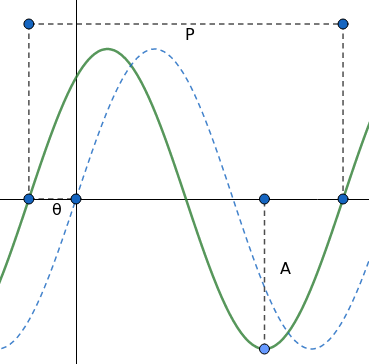
\includegraphics[scale=0.6]{fig/img/AC.png}
	\caption{Two ACs, $i(t)=A\sin(\omega t)$ and $i(t)=A\sin(\omega t+\theta)$ shown in a dotted blue line and a green, respectively. The current shown in green has been phase shifted by $\theta$. The currents have amplitude $A$, and period $P=f^{-1}$.}
\end{figure}
\noindent A certain type of AC exists, where the current is constant for half a period, and then turned off for the other half. This type of AC is called a step voltage, and the graph for this can be seen in figure \ref{fig:AC_step}.
\begin{figure}[H] 
\begin{center}
\begin{tikzpicture}
\begin{axis}[ticks=none,
axis lines =center,
xlabel={t},
ylabel={i(t)},
    height=7cm, width=9cm,
    xmin=0, xmax=10, ymin=-2, ymax=2]
\addplot [
    domain=0:3.14, 
    samples=100, 
    color=red,
]
{1};
\addplot +[mark=none, color=red] coordinates {(3.14, 0) (3.14, 1)};
\addplot [
    domain=3.14:6.28, 
    samples=100, 
    color=red,
    ]
    {0)};
\addplot +[mark=none, color=red] coordinates {(2*3.14, 0) (2*3.14, 1)};
\addplot [
    domain=6.28:9.42, 
    samples=100, 
    color=red,
]
{1};
\addlegendentry{AC step input}
\end{axis}
\end{tikzpicture}
\end{center}
\caption{AC step current versus time}
\label{fig:AC_step}
\end{figure}
\section{Voltage}
Voltage ($v$) is defined as the amount of work that it requires to move a charge of $1 C$ through an element. This is expressed in the following equation: \cite[p. 8]{bcircuit}
\begin{align*}
	v=\dfrac{dw}{dq},
\end{align*}
\\
where $w$ is the work (in watts, $W$).
\section{Resistor}
When a resistor, which is a passive element, is added to a circuit, it creates a resistance ($R$, in ohms, $\Omega$). Resistance makes it more difficult for the current to pass through the element. Resistance is defined as the proportional constant between current and voltage. The mathematical relation of this is given by: \cite[p.~22]{bcircuit5}
\begin{align} 
\label{Ohm}
v(t)=R\cdot i(t),\ R\geq0,
\end{align}
\section{Power} 
Power ($p$) measures energy exerted per second (in watts, $W$). Power can be expressed as: \cite[p. 22]{bcircuit5}.
\begin{align} 
\label{power}
p(t)=v(t)\cdot i(t).
\end{align}
By inserting this in equation \eqref{Ohm}, the following expression is found:
\begin{align}
p(t)=\dfrac{v^2(t)}{R}. \label{resistor:power}
\end{align}

\section{Capacitor}
A capacitor, which is a passive element, consists of two similar sized plates with a distance between them. When a current is applied to the circuit, the capacitor gets charged. The capacitance ($C$) is the amount of energy a capacitor can store, when it is fully charged. The capacitor gets charged, when a positive charge is transferred from one plate to another through the circuit.
\\
The capacitance is given by the following equation:
\begin{align*}
C=\dfrac{\epsilon_{0}A}{d},
\end{align*}
where $C$ is the capacitance (in farad, $F$), and $\epsilon_{0}$ is the permittivity of free space, which is equal to $8.85 \cdot 10^{-12}                                                 \frac{F}{m}$. $A$ is the surface area of the plates (in square meters, $m^{2}$), and $d$ is the distance between the two plates (in meters, $m$).
\\
The charge of a capacitor across a voltage ($v$) and capacitance ($C$) is equal to: \cite[p.~253]{bcircuit5}
\begin{align}
\label{QCV}
q_C(t) = Cv_C(t).	
\end{align}
From \eqref{I=dq/dt}, current is defined as:
\begin{align*}
	i(t) = \frac{dq(t)}{dt}.
\end{align*}
The current across a capacitor is then:
\begin{align*}
	i_C(t) = \frac{d}{dt}\big(Cv_C(t)\big).
\end{align*}
For a capacitor with capacitance ($C$), the current across the capacitor can be written as:
\begin{align}
	i_C(t) = C\frac{dv_C(t)}{dt}.\label{iC}
\end{align}
\section{Time constant}
When describing the charging and discharging of a capacitor, $\tau$ is a useful constant. The product of the resistance ($R$) and the capacitance ($C$) is called the time constant, $R \cdot C = \tau$.

\section{Circuit diagrams}
Electrical circuits are visually represented in circuit diagrams. In addition to the above-mentioned elements, the circuit diagrams introduce three terms: nodes, branches, and loops. Elements are \textit{branches}, i.e.  the voltage supply, resistors, capacitors, and the like. \textit{Nodes} connect the \textit{branches} of the circuit. Lastly, any closed path in the circuit, in which no node is encountered more than than once, is called a \textit{loop} \cite[page~32]{bcircuit}. An example of a circuit is shown below.

\begin{figure}[H]
 \begin{center}
\begin{circuitikz}[american voltages]
\draw
to[battery, battery1=$V_{B}$, color=blue] (0,2)
to[resistor, R=$R_1$, color=red] (2,2)
to[resistor, R=$R_2$, color=red] (2,0)
to[short, -] (0,0)
[short, -](2,2) to [short, -] (3,2)
to[resistor, R=$R_3$, color=red](3,0)
to[short, -] (2,0)
[short](3,2) to [short] (5,2)
to [C=$C$, color=green](5,0)
to [short, -] (3,0)
(0,0) to [short, l_=$N_3$, -] (5,0)
(2,2) to [short, l^=$N_2$, -] (5,2)
(0,1) to [short, l^=$N_1$, -] (0,2);
\end{circuitikz}
\end{center}
 \caption{A circuit with a battery, three resistors and a light bulb}
\end{figure}

\noindent This circuit has five branches, which are shown marked in color: a battery (in blue), three resistors ($R_1, R_2,$ and $R_3$, in red), and the light bulb (in green). The three nodes of the circuit ($N_1$, $N_2$, and $N_3$) connect the branches. Additionally, there are three loops, all of which have the same starting and ending point, $V_{battery}$. The first loop passes through $R_2$ and $R_1$, and returns to the starting point. Similarly, the second loop passes through $R_3$ and $R_1$, and returns. The third, and final, loop runs through the light bulb, then $R_1$, and returns. 

\subsection{Kirchhoff's laws}\label{Klaws}
\textbf{Kirchhoff's current law (KCL)}
\\
Observe a circuit up until a node, past which the path of the circuit splits in two. The current encountering the node does not accumulate (as it would, e.g. in a battery). Instead, all electrons flowing to that node split up between the available paths, and continue to flow through the circuit. This is Kirchhoff’s current law (KCL), which states that the algebraic sum of all currents in a node is equal to zero:
\begin{align}
\sum_{j=1}^{N} i_{j}(t) = 0,
\end{align}
where $i_{j}(t)$ is the $j$'th current entering the node through branch $j$, with $N$ branches connected to the node. \cite[page~32]{bcircuit}
\\
\\
\textbf{Kirchhoff's voltage law (KVL)}
\\
Kirchhoff's voltage law states that the algebraic sum of all voltages in a loop is equal to zero. This can be expressed mathematically as:
\begin{align}
\sum_{j=1}^{N} v_{j}(t) = 0,
\end{align}
where $v_{j}(t)$ is the voltage in the $j$'th voltage with $N$ voltages. \citep[page~34]{bcircuit}\\

